% Options for packages loaded elsewhere
\PassOptionsToPackage{unicode}{hyperref}
\PassOptionsToPackage{hyphens}{url}
\PassOptionsToPackage{dvipsnames,svgnames,x11names}{xcolor}
\documentclass[
  11pt,
]{article}
\usepackage{xcolor}
\usepackage[margin=1in]{geometry}
\usepackage{amsmath,amssymb}
\setcounter{secnumdepth}{-\maxdimen} % remove section numbering
\usepackage{iftex}
\ifPDFTeX
  \usepackage[T1]{fontenc}
  \usepackage[utf8]{inputenc}
  \usepackage{textcomp} % provide euro and other symbols
\else % if luatex or xetex
  \usepackage{unicode-math} % this also loads fontspec
  \defaultfontfeatures{Scale=MatchLowercase}
  \defaultfontfeatures[\rmfamily]{Ligatures=TeX,Scale=1}
\fi
\usepackage{lmodern}
\ifPDFTeX\else
  % xetex/luatex font selection
\fi
% Use upquote if available, for straight quotes in verbatim environments
\IfFileExists{upquote.sty}{\usepackage{upquote}}{}
\IfFileExists{microtype.sty}{% use microtype if available
  \usepackage[]{microtype}
  \UseMicrotypeSet[protrusion]{basicmath} % disable protrusion for tt fonts
}{}
\makeatletter
\@ifundefined{KOMAClassName}{% if non-KOMA class
  \IfFileExists{parskip.sty}{%
    \usepackage{parskip}
  }{% else
    \setlength{\parindent}{0pt}
    \setlength{\parskip}{6pt plus 2pt minus 1pt}}
}{% if KOMA class
  \KOMAoptions{parskip=half}}
\makeatother
\usepackage{longtable,booktabs,array}
\usepackage{calc} % for calculating minipage widths
% Correct order of tables after \paragraph or \subparagraph
\usepackage{etoolbox}
\makeatletter
\patchcmd\longtable{\par}{\if@noskipsec\mbox{}\fi\par}{}{}
\makeatother
% Allow footnotes in longtable head/foot
\IfFileExists{footnotehyper.sty}{\usepackage{footnotehyper}}{\usepackage{footnote}}
\makesavenoteenv{longtable}
\usepackage{graphicx}
\makeatletter
\newsavebox\pandoc@box
\newcommand*\pandocbounded[1]{% scales image to fit in text height/width
  \sbox\pandoc@box{#1}%
  \Gscale@div\@tempa{\textheight}{\dimexpr\ht\pandoc@box+\dp\pandoc@box\relax}%
  \Gscale@div\@tempb{\linewidth}{\wd\pandoc@box}%
  \ifdim\@tempb\p@<\@tempa\p@\let\@tempa\@tempb\fi% select the smaller of both
  \ifdim\@tempa\p@<\p@\scalebox{\@tempa}{\usebox\pandoc@box}%
  \else\usebox{\pandoc@box}%
  \fi%
}
% Set default figure placement to htbp
\def\fps@figure{htbp}
\makeatother
\setlength{\emergencystretch}{3em} % prevent overfull lines
\providecommand{\tightlist}{%
  \setlength{\itemsep}{0pt}\setlength{\parskip}{0pt}}
% House preamble for 034_higher_cell_cochain_projection_and_retraction_dynamics
%
% Typesetting is not evidence for any claim.
%
% Reviewed 2026-10-02.
%
% xelatex, not pdflatex: the manuscript uses unicode characters that pdflatex
% cannot set without per-character declarations.

\usepackage{fontspec}
\usepackage{unicode-math}
\setmainfont{lmroman10-regular.otf}[BoldFont=lmroman10-bold.otf,ItalicFont=lmroman10-italic.otf,BoldItalicFont=lmroman10-bolditalic.otf]
\setmonofont{lmmono10-regular.otf}[Scale=0.85]
\setmathfont{latinmodern-math.otf}

\usepackage{amsmath,amssymb,amsthm}
\usepackage[margin=1in]{geometry}
\usepackage{longtable,booktabs,array}
\usepackage{microtype}
\usepackage{enumitem}
\setlist{nosep,leftmargin=1.4em}

\usepackage[dvipsnames]{xcolor}
\usepackage[colorlinks=true,linkcolor=RoyalBlue,urlcolor=RoyalBlue,
            citecolor=RoyalBlue,breaklinks=true]{hyperref}
\usepackage{fvextra}
\usepackage{framed}
\fvset{breaklines=true,breakanywhere=true,fontsize=\small}

\AtBeginEnvironment{longtable}{\small}
\setlength{\tabcolsep}{4pt}
\renewcommand{\arraystretch}{1.15}

\providecommand{\tightlist}{%
  \setlength{\itemsep}{0pt}\setlength{\parskip}{0pt}}

\definecolor{quoterule}{gray}{0.75}
\renewenvironment{quote}
  {\begin{leftbar}\small}
  {\end{leftbar}}

\usepackage[htt]{hyphenat}
\usepackage{xurl}
\emergencystretch=3em
\sloppy

\usepackage{seqsplit}
\usepackage{bookmark}
\IfFileExists{xurl.sty}{\usepackage{xurl}}{} % add URL line breaks if available
\urlstyle{same}
\hypersetup{
  pdftitle={Higher-Cell Product Retractions, Simplicial Cochains, and Finite Retraction Dynamics},
  pdfauthor={Jeremy H. Carroll},
  colorlinks=true,
  linkcolor={RoyalBlue},
  filecolor={Maroon},
  citecolor={Blue},
  urlcolor={Blue},
  pdfcreator={LaTeX via pandoc}}

\title{Higher-Cell Product Retractions, Simplicial Cochains, and Finite Retraction Dynamics}
\author{Jeremy H. Carroll}
\date{Technical preprint v0.1, 2026-10-10}

\begin{document}
\maketitle

\textbf{Series:} 002\_PROJECTION\_OBSTRUCTION (PO-034)\\
\textbf{Version:} v0.1 (0.1.0), technical preprint candidate\\
\textbf{Status:} Unpublished technical preprint; first publication review candidate; deposition not verified\\
\textbf{License:} CC-BY-4.0 for the manuscript; PolyForm Noncommercial 1.0.0 for code and Lean sources\\
\textbf{Authority effect:} None

\subsection{Abstract}\label{abstract}

Product-of-marginals retraction gives a finite diagnostic for departure from a fully factorized quantum-state model. At a product reference state, its derivative is an idempotent oblique projector that preserves every single-site marginal. We distinguish its complementary residual from a different projector onto the highest-order tensor component. Single-site Hamiltonian terms are tangent, whereas a two-site interaction can generate a nonzero product-state residual inside a three-site cell. A worked counterexample corrects the stronger isolation claim in the earlier candidate.

For a finite, closed system with product initial data and a bound on the operator norm of the entire Hamiltonian, we derive a quadratic lower bound on distance to the product of marginals. Lemma 4.3a refines that coefficient by the site budgets of a declared interaction decomposition. Lemma 4.3b carries the same coefficient to the reduced state on a declared subsystem of a finite dilation. The global norm remains in the coefficient. Lemma 4.3c treats one jump generator with no finite autonomous Hermitian dilation. Lemma 4.3d gives a coarser quadratic coefficient for a finite family of jumps and no Hamiltonian; on the Lemma 4.3c data the coefficient is \(10\), not \(6\). Lemma 4.3e puts a bounded Hamiltonian beside that family. The quadratic coefficient is \(2(1+k^2)(g+G)^2\). On a commuting witness with \(g=G=1\) and \(k=2\) it equals \(40\), not \(6\). Lemma 4.3f shows that the state-acceleration bound used for that square cannot replace \((g+G)^2\) by \(g^2+G^2\): a product witness has \(\|\rho''(0)\|_1=10>8\), while \(D(t)=0\). This distance measures total failure of factorization, including classical correlations; nonzero distance alone does not establish entanglement or genuine multipartite entanglement. For two qubits, however, distance greater than one is sufficient for entanglement (Hall, 2013). We then give the explicit observation needed to turn residuals into simplicial cochains, review finite scalar Hodge decomposition, fix a graded-square sign convention, and derive a separate state-local semigroup defect coefficient. No identity between these two defects is assumed. The package supplies numerical examples and conditional abstract Lean proofs of projector identities. Evidence scope and unfinished formal replay obligations are stated explicitly.

\subsection{1. Scope, notation, and contribution}\label{scope-notation-and-contribution}

All Hilbert spaces, matrices, simplicial complexes, and examples in this paper are finite. The contribution is a consistent account of which projection diagnostic answers which question, with proofs, counterexamples, and a reproducible computational package. The basic projector and Hodge identities are standard finite algebra; this paper does not claim a new complete theory of topology or non-Abelian geometry.

Two indices must remain separate:

\begin{longtable}[]{@{}
  >{\raggedright\arraybackslash}p{(\linewidth - 4\tabcolsep) * \real{0.3333}}
  >{\raggedright\arraybackslash}p{(\linewidth - 4\tabcolsep) * \real{0.3333}}
  >{\raggedright\arraybackslash}p{(\linewidth - 4\tabcolsep) * \real{0.3333}}@{}}
\toprule\noalign{}
\begin{minipage}[b]{\linewidth}\raggedright
Symbol
\end{minipage} & \begin{minipage}[b]{\linewidth}\raggedright
Meaning
\end{minipage} & \begin{minipage}[b]{\linewidth}\raggedright
Three-site example
\end{minipage} \\
\midrule\noalign{}
\endhead
\bottomrule\noalign{}
\endlastfoot
\(k\) & Number of quantum subsystems in a support \(\sigma\) & \(k=3\) \\
\(p\) & Simplicial dimension and cochain degree & \(p=k-1=2\) \\
\(q\) & An independently declared memory grade & Not a subsystem count \\
\(Q\) & Complement of the fully factorized tangent projector & Retains two-site and three-site components \\
\(R_k\) & Highest-order reference-dependent component projector & Removes proper-support components \\
\end{longtable}

An abstract \(p\)-simplex has \(p+1\) vertices. A hyperedge of cardinality \(k\) does not by itself supply a simplicial boundary: one must declare a complex containing its faces.

Here a \textbf{finite autonomous Hermitian dilation} means one fixed
finite-dimensional total carrier, one fixed time-independent Hermitian
Hamiltonian, and one fixed initial total state whose reduction reproduces
the entire specified trajectory for every \(t\ge0\). The no-go statements
in Lemmas 4.3c and 4.3f use this meaning. They do not address time-by-time
dilations or unrestricted time-dependent Hamiltonians.

The paper assigns no operational authorization or institutional standing. A mathematical witness, an integrity check, and a policy decision have different meanings.

\subsection{2. Product retraction and its derivative}\label{product-retraction-and-its-derivative}

Let \(\sigma=\{1,\ldots,k\}\), with \(k\ge2\), and let
\[
\mathcal H_\sigma=\bigotimes_{j=1}^k\mathcal H_j,\qquad
\dim\mathcal H_j=d_j<\infty.
\]
Write \(\tau_j Z=\operatorname{Tr}_{\sigma\setminus\{j\}}Z\).
Density matrices are positive semidefinite Hermitian matrices of trace one.
The ambient affine space is the trace-one Hermitian space; its translation space
\(\mathcal B_0\) consists of traceless Hermitian matrices.

For a density matrix \(S\), define
\[
\Pi(S)=\bigotimes_{j=1}^k\tau_j S.
\]
This map preserves the single-site marginals and fixes every product density.
At a reference
\(\rho=\bigotimes_j\rho_j\), with \(\operatorname{Tr}\rho_j=1\), write
\[
\iota_j z_j=
\rho_1\otimes\cdots\otimes\rho_{j-1}\otimes z_j
\otimes\rho_{j+1}\otimes\cdots\otimes\rho_k.
\]
For \(Z\in\mathcal B_0\), differentiation on the trace-one affine space gives
\[
PZ=D\Pi_\rho Z=\sum_{j=1}^k\iota_j(\tau_j Z),\qquad Q=I-P.
\]

\subsubsection{2.1 Boundary states and the full-space extension}\label{boundary-states-and-the-full-space-extension}

For full-rank factors, the product densities form a smooth manifold locally.
At pure or rank-deficient factors, positivity introduces a boundary.
At any product reference, \(\operatorname{im}P\) is the tangent space of the smooth algebraic product manifold formed from normalized Hermitian factors; \(\mathcal B_0\) is the ambient variation space. It is not the set of all feasible two-sided density-matrix velocities at a boundary point.

The software accepts arbitrary matrix perturbations through a separately
declared homogeneous extension, defined near \(\operatorname{Tr}S=1\):
\[
\widehat\Pi(S)=(\operatorname{Tr}S)^{1-k}
              \bigotimes_j\tau_j S.
\]
Its derivative is
\[
\widehat PZ=\sum_j\iota_j(\tau_j Z)
            -(k-1)\operatorname{Tr}(Z)\rho.
\]
It restricts to \(P\) on trace-zero directions. Its full-space image contains
the radial direction \(\rho\) as well as the algebraic tangent space.
The correction term is not the unrestricted derivative of the unnormalized
map \(S\mapsto\bigotimes_j\tau_j S\). The code applies it linearly, without a
trace-dependent numerical threshold.

\subsection{3. Projector identities and the locality correction}\label{projector-identities-and-the-locality-correction}

\subsubsection{Theorem 4.1 (Idempotence, marginals, and kernel)}\label{theorem-4.1-idempotence-marginals-and-kernel}

On \(\mathcal B_0\),
\[
P^2=P,\qquad \tau_j(PZ)=\tau_j Z,
\]
and
\[
\operatorname{im}P
 =\left\{\sum_j\iota_j z_j:\ z_j=z_j^\dagger,\
                 \operatorname{Tr}z_j=0\right\},
\qquad
\ker P=\{Z:\tau_j Z=0\ \text{for every }j\}.
\]
The image is the algebraic product tangent space described in Section 2.1.

\textbf{Proof.} For trace-zero \(z_j\), normalization of the other factors gives
\[
\tau_l(\iota_j z_j)=
\begin{cases}
z_j,&l=j,\\
0,&l\ne j.
\end{cases}
\]
Since \(\operatorname{Tr}\tau_j Z=\operatorname{Tr}Z=0\), this identity
immediately gives marginal preservation. Applying it twice gives \(P^2Z=PZ\).
Each \(PZ\) lies in the displayed sum, and \(P\) fixes every vector in that sum.
Finally, \(PZ=0\) implies \(\tau_j Z=\tau_j(PZ)=0\); the converse follows
from the definition. \(\square\)

Consequently, \(Q^2=Q\), \(PQ=QP=0\), and every single-site marginal of \(QZ\)
vanishes. The term ``normal'' refers to the chosen complementary subspace;
an oblique \(P\) need not define an orthogonal projection.

\subsubsection{Theorem 4.2 (One-site tangent isolation)}\label{theorem-4.2-one-site-tangent-isolation}

For a Hermitian operator \(h_j\) acting only on site \(j\),
\[
Q\bigl(-i[h_j\otimes I_{\sigma\setminus\{j\}},\rho]\bigr)=0.
\]

\textbf{Proof.} The commutator is
\(\iota_j(-i[h_j,\rho_j])\), whose local factor has trace zero.
Theorem 4.1 fixes this elementary tangent vector. Linearity also annihilates
any sum of one-site commutators. \(\square\)

This theorem does not extend to every interaction with support smaller
than \(k\). For \(X\subsetneq\sigma\),
\[
-i[h_X\otimes I,\rho]
 =-i[h_X,\rho_X]\otimes\rho_{\sigma\setminus X},
\]
but \(-i[h_X,\rho_X]\) need not be a sum of one-site variations.

\subsubsection{Counterexample 4.2a (Two-site residual inside a triangle)}\label{counterexample-4.2a-two-site-residual-inside-a-triangle}

Let \(k=3\), \(\rho=|000\rangle\langle000|\), and
\(H=X_1X_2\otimes I_3\), where \(X\) is Pauli \(X\).
Then
\[
L=-i[H,\rho]
 =-i\bigl(|110\rangle\langle000|-|000\rangle\langle110|\bigr).
\]
Every single-site marginal of \(L\) is zero. Thus
\[
PL=0,\qquad QL=L,\qquad \|QL\|_1=2.
\]
The support has size two, strictly smaller than three. The spectator-site
marginal is zero, but that fact does not establish \(QL=0\).
At later times the state is a correlated two-qubit state tensored with
\(|0\rangle\langle0|\); it has no genuine three-party entanglement.

Full support is also insufficient for a nonzero residual: any Hamiltonian
commuting with the reference state has \(L=0\).

\subsubsection{Proposition 4.2b (A distinct highest-order projector)}\label{proposition-4.2b-a-distinct-highest-order-projector}

Let \(E_j Z\) replace subsystem \(j\) by \(\rho_j\), retaining the reduced
operator on all other subsystems, with tensor factors restored to their
declared order:
\[
E_j Z=\rho_j\otimes_j\operatorname{Tr}_j Z,\qquad
R_k=\prod_{j=1}^k(I-E_j).
\]
Here \(\otimes_j\) means insertion at site \(j\).
The \(E_j\) are commuting idempotents: \(E_j^2=E_j\) and
\(E_iE_j=E_jE_i\). Therefore \(R_k^2=R_k\).
If \(Z=Z_X\otimes\rho_{\sigma\setminus X}\) for a proper subset \(X\),
choose \(j\notin X\). Then \(E_jZ=Z\), so \(R_kZ=0\).
This establishes proper-support annihilation for \textbf{\(R_k\)}.

The highest-order projector selects the tensor component with a traceless
local factor at every site. It is reference-dependent and is not a connected
information measure; its nonzero value alone is not an entanglement witness. For \(k=2\), it agrees with
\(Q\) on trace-zero perturbations. For \(k>2\), \(Q\) also retains intermediate
orders. In Counterexample 4.2a, \(R_3L=0\) while \(QL=L\).

\subsection{4. Short-time distance and dual witnesses}\label{short-time-distance-and-dual-witnesses}

\subsubsection{Theorem 4.3 (A finite-Hamiltonian lower bound)}\label{theorem-4.3-a-finite-hamiltonian-lower-bound}

Let \(H=H^\dagger\) act on the closed finite system \(\mathcal H_\sigma\).
Assume \(\|H\|_\infty\le g\), \(g>0\), and product initial data \(\rho(0)=\rho\).
Set
\[
\rho(t)=e^{-itH}\rho e^{itH},\quad
D(t)=\|\rho(t)-\Pi(\rho(t))\|_1,\quad
\nu=\|Q(-i[H,\rho])\|_1.
\]
For every \(t\ge0\),
\[
D(t)\ge\nu t-2(1+k^2)g^2t^2
       \ge\nu t-6k^2g^2t^2.
\]
If \(\nu>0\) and \(0\le t\le t_*=\nu/(12k^2g^2)\), then
\(D(t)\ge\nu t/2\), strictly positive for \(t>0\).

\textbf{Proof.} Unitary invariance of the trace norm and the commutator estimate
\(\|[H,Z]\|_1\le2\|H\|_\infty\|Z\|_1\) imply uniformly in time
\[
\|\rho'(t)\|_1\le2g,\qquad
\|\rho''(t)\|_1\le4g^2.
\]
Partial trace is trace-norm contractive on Hermitian inputs, so each
single-site marginal obeys the same two bounds. Every marginal density has
trace norm one. Differentiating
\(F(t)=\bigotimes_j\rho_j(t)\), and using trace-norm multiplicativity on
tensor products, yields
\[
\begin{aligned}
\|F''(t)\|_1
&\le \sum_j\|\rho_j''(t)\|_1
 +\sum_{i\ne j}\|\rho_i'(t)\|_1\|\rho_j'(t)\|_1\\
&\le4kg^2+4k(k-1)g^2=4k^2g^2.
\end{aligned}
\]
For \(f(t)=\rho(t)-F(t)\), we have \(f(0)=0\), \(f'(0)=n=QL\), and
\(\|f''(t)\|_1\le4(1+k^2)g^2\). The integral remainder gives
\[
f(t)=tn+\int_0^t(t-s)f''(s)\,ds,\qquad
\|f(t)-tn\|_1\le2(1+k^2)g^2t^2.
\]
The reverse triangle inequality establishes the first bound; the second is
weaker for \(k\ge2\). The stated window makes the weaker quadratic term
at most \(\nu t/2\). \(\square\)

Here \(g\) bounds the \textbf{whole Hamiltonian}, not
\(\max_j\sum_{X\ni j}\|h_X\|_\infty\).
An interaction decomposition supplies a valid, possibly loose choice
\(g=\sum_X\|h_X\|_\infty\). Lemma 4.3a is the closed-system refinement
that uses the site budgets of a declared decomposition. The global norm
remains in the coefficient. Lemma 4.3b extends that coefficient to the
reduced state of a declared subsystem inside a finite dilation. Lemma 4.3c
is one jump trajectory with no finite autonomous Hermitian dilation. Lemma 4.3d
gives a quadratic coefficient for a finite family of jumps and no
Hamiltonian. On the Lemma 4.3c data that coefficient is \(10\), not the
scalar coefficient \(6\). Lemma 4.3e puts a bounded Hamiltonian beside
that family. The quadratic coefficient is \(2(1+k^2)(g+G)^2\). It is
not the scalar coefficient \(6\). Lemma 4.3f shows that the
acceleration estimate producing the square cannot replace
\((g+G)^2\) by \(g^2+G^2\). The defect coefficient is unchanged.

\subsubsection{Lemma 4.3a (Site-budget refinement on a closed system)}\label{lemma-4.3a-site-budget-refinement-on-a-closed-system}

Let
\[
H=\sum_{\alpha=1}^{N}h_\alpha
\]
on the closed finite system \(\mathcal H_\sigma\), where each
\(h_\alpha=h_\alpha^\dagger\) is supported on a declared subset
\(X_\alpha\subseteq\sigma\) and is extended by the identity on the
complement. Let \(g\ge\|H\|_\infty\) and
\[
g_j=\sum_{\alpha:\,j\in X_\alpha}\|h_\alpha\|_\infty.
\]
Keep the product initial state, \(D\), \(\nu\), and
\(f(t)=\rho(t)-\bigotimes_j\rho_j(t)\) of Theorem 4.3. Set
\[
\Gamma
=g^2+g\sum_{j=1}^k g_j+\sum_{i\ne j}g_ig_j.
\]
Then, for every \(t\ge0\),
\[
D(t)\ge\nu t-2\Gamma t^2.
\]
If \(\nu>0\) and \(0\le t\le\nu/(4\Gamma)\), then \(D(t)\ge\nu t/2\).

On the one-term decomposition \(h_1=H\), with declared support \(X_1=\sigma\) and \(g=\|H\|_\infty\), one has
\(g_j=g\) and \(\Gamma=(1+k^2)g^2\), so the quadratic coefficient equals
the leading coefficient of Theorem 4.3. A decomposition with some
\(g_j<g\) can make \(\Gamma\) strictly smaller. A redundant decomposition
can make \(\Gamma\) larger. Theorem 4.3 remains available unchanged.

\textbf{Proof.} If \(K=I_j\otimes A\) on \(\mathcal H_j\otimes\mathcal H_R\),
with \(R=\sigma\setminus\{j\}\), then \(\tau_j([K,Z])=0\) for every
matrix \(Z\). In a product basis the kept matrix element is
\[
\sum_b[K,Z]_{(ab),(a'b)}
=\sum_{b,b''}A_{bb''}Z_{(ab''),(a'b)}
-\sum_{b,b''}Z_{(ab),(a'b'')}A_{b''b}.
\]
Renaming \(b''\leftrightarrow b\) in the second sum produces the first,
because the scalar matrix elements of \(A\) commute with those of \(Z\).
Terms of \(H\) supported off site \(j\) therefore drop out:
\[
\tau_j([H,Z])
=\tau_j\Bigl(\Bigl[\sum_{j\in X_\alpha}h_\alpha,\,Z\Bigr]\Bigr).
\]
The commutator estimate
\(\|[B,Z]\|_1\le2\|B\|_\infty\|Z\|_1\) and trace-norm contractivity of
the partial trace on Hermitian inputs give
\(\|\rho'(t)\|_1\le2g\) and \(\|\rho''(t)\|_1\le4g^2\), as in Theorem 4.3.
The same two facts, applied only to the terms that meet site \(j\) and
using \(\|\rho(t)\|_1=1\), give \(\|\rho_j'(t)\|_1\le2g_j\). Since
\(\rho_j''=\tau_j(-i[H,\rho'])\) and \(\|\rho'(t)\|_1\le2g\),
\[
\|\rho_j''(t)\|_1
\le\sum_{j\in X_\alpha}2\|h_\alpha\|_\infty\|\rho'(t)\|_1
\le4gg_j.
\]
Every marginal density has trace norm one.
The product rule and trace-norm multiplicativity give
\[
\begin{aligned}
\|F''(t)\|_1
&\le\sum_j4gg_j+\sum_{i\ne j}(2g_i)(2g_j)\\
&=4g\sum_jg_j+4\sum_{i\ne j}g_ig_j.
\end{aligned}
\]
Hence \(\|f''(t)\|_1\le4\Gamma\). As in Theorem 4.3,
\(f(t)=tn+\int_0^t(t-s)f''(s)\,ds\), so the remainder has trace norm at
most \(4\Gamma\cdot t^2/2=2\Gamma t^2\). The reverse triangle inequality
gives the bound.
If \(\nu>0\), then \(\|H\|_\infty>0\), so \(g>0\) and \(\Gamma\ge g^2>0\).
The stated window makes the quadratic term at most \(\nu t/2\).
The one-term identities are substitutions. \(\square\)

The factor \(g\) in \(\Gamma\) is the global operator-norm budget. The
lemma does not replace it by \(\max_j g_j\). If the state on \(\sigma\)
is only the reduction of a larger closed system, this closed-system
argument does not apply by itself. Lemma 4.3b treats that reduction
when a finite autonomous Hermitian dilation is declared. Neither lemma removes
\(g\).

\subsubsection{Example 4.3a (A strictly sharper coefficient)}\label{example-4.3a-a-strictly-sharper-coefficient}

Take \(k=3\), \(\rho=|000\rangle\langle000|\), and
\(H=X\otimes X\otimes I\), so \(\|H\|_\infty=1\). Use the one-term
decomposition supported on \(\{1,2\}\), with \(g=1\), \(g_1=g_2=1\),
and \(g_3=0\). Then
\[
\sum_j g_j=2,\qquad
\sum_{i\ne j}g_ig_j=2,\qquad
\Gamma=5.
\]
The quadratic coefficient is \(2\Gamma=10\). Theorem 4.3 with the same
\(g\) has leading coefficient \(2(1+k^2)g^2=20\). The exact state is
\[
|\psi(t)\rangle=\cos t\,|000\rangle-i\sin t\,|110\rangle.
\]
The site-3 marginal is \(|0\rangle\langle0|\) for every \(t\), so its
velocity has trace norm \(0=2g_3\). The site-1 marginal is
\(\operatorname{diag}(\cos^2 t,\sin^2 t)\), with
\[
\|\rho_1'(t)\|_1=2|\sin(2t)|,
\]
equal to \(2g_1\) at \(t=\pi/4\). Counterexample 4.2a gives \(\nu=2\).
Thus \(D(t)\ge2t-10t^2\), and \(D(t)\ge t\) for \(0\le t\le1/10\).
The published Theorem 4.3 window on these data, using the weaker
coefficient \(54g^2\), is only \(0\le t\le1/54\).

This example is an exact symbolic witness. It is not a Python test, and
it does not evaluate \(D(t)\) itself. The code path for Theorem 4.3 is
unchanged and still uses the weaker coefficient.

\subsubsection{Lemma 4.3b (Reduced site-budget bound on a finite dilation)}\label{lemma-4.3b-reduced-site-budget-bound-on-a-finite-dilation}

Let the closed finite carrier be the disjoint union
\(\sigma\sqcup\varepsilon\), with \(k=|\sigma|\ge 2\) and \(\varepsilon\)
nonempty. Let
\[
H=\sum_{\alpha=1}^{N}h_\alpha
\]
be Hermitian on \(\mathcal H_\sigma\otimes\mathcal H_\varepsilon\), where
each \(h_\alpha=h_\alpha^\dagger\) is supported on a declared subset
\(X_\alpha\) of the full site set and is extended by the identity off
that subset. Let \(g\ge\|H\|_\infty\) and, for each system site
\(j\in\sigma\),
\[
g_j=\sum_{\alpha:\,j\in X_\alpha}\|h_\alpha\|_\infty.
\]
A term supported only on \(\varepsilon\) contributes to no system budget
\(g_j\). Let
\[
\rho_{\mathrm{tot}}(t)=e^{-itH}\rho_{\mathrm{tot}}(0)e^{itH},\qquad
\rho_\sigma(t)=\tau_\varepsilon(\rho_{\mathrm{tot}}(t)),
\]
and write \(\rho_j(t)\) for the single-site marginal of
\(\rho_\sigma(t)\). Assume
\(\rho_\sigma(0)=\bigotimes_{j\in\sigma}\rho_j(0)\). Set
\(f(t)=\rho_\sigma(t)-\bigotimes_{j\in\sigma}\rho_j(t)\),
\[
D_\sigma(t)=\|f(t)\|_1,\qquad
\nu_\sigma=\|f'(0)\|_1,
\]
and
\[
\Gamma
=g^2+g\sum_{j\in\sigma}g_j+\sum_{\substack{i,j\in\sigma\\ i\ne j}}g_ig_j.
\]
Then, for every \(t\ge 0\),
\[
D_\sigma(t)\ge\nu_\sigma t-2\Gamma t^2.
\]
If \(\nu_\sigma>0\) and \(0\le t\le\nu_\sigma/(4\Gamma)\), then
\(D_\sigma(t)\ge\nu_\sigma t/2\).

If instead \(H=H_\sigma\otimes I_\varepsilon+I_\sigma\otimes H_\varepsilon\),
then for every initial total state
\[
\rho_\sigma(t)=e^{-itH_\sigma}\rho_\sigma(0)e^{itH_\sigma}.
\]
The norm of \(H_\varepsilon\) does not appear in this trajectory. When
\(\rho_\sigma(0)\) is a site product and \(g\ge\|H_\sigma\|_\infty\),
Lemma 4.3a applies on \(\sigma\) with the site budgets of \(H_\sigma\)
alone.

The factor \(g\) remains in \(\Gamma\). The lemma does not replace it
by \(\max_j g_j\). A reduced generator supplied only as a Lindblad map,
without a finite autonomous Hermitian dilation and a declared norm bound, is not
covered. An environment-only summand can make the admitted \(g\) larger
than the norm of a particular reduced generator.

\textbf{Proof.} Lemma 4.3a's single-site identity, applied on the dilated
carrier, gives
\(\tau_j([H,Z])=\tau_j([\sum_{j\in X_\alpha}h_\alpha,Z])\)
for every matrix \(Z\). Partial trace is trace-norm contractive on
Hermitian inputs, and
\(\|[B,Z]\|_1\le 2\|B\|_\infty\|Z\|_1\). Hence
\(\|\rho_{\mathrm{tot}}'(t)\|_1\le 2g\) and
\(\|\rho_{\mathrm{tot}}''(t)\|_1\le 4g^2\), and the contracted system
derivatives obey the same two bounds. Keeping only the terms that meet
system site \(j\), and using
\(\|\rho_{\mathrm{tot}}'(t)\|_1\le 2g\), gives
\(\|\rho_j'(t)\|_1\le 2g_j\) and \(\|\rho_j''(t)\|_1\le 4gg_j\).

Every system marginal is a density matrix. Differentiating
\(F(t)=\bigotimes_{j\in\sigma}\rho_j(t)\) and using trace-norm
multiplicativity, as in Theorem 4.3, yields
\[
\|F''(t)\|_1
\le\sum_{j\in\sigma}4gg_j+\sum_{\substack{i,j\in\sigma\\ i\ne j}}4g_ig_j.
\]
Thus \(\|f''(t)\|_1\le 4\Gamma\). The integral remainder gives
\(f(t)=tf'(0)+\int_0^t(t-s)f''(s)\,ds\), so the remainder has trace
norm at most \(2\Gamma t^2\). The reverse triangle inequality is the
bound. If \(\nu_\sigma>0\), then \(\|H\|_\infty>0\), so \(g>0\) and
\(\Gamma\ge g^2>0\). The stated window makes the quadratic term at most
\(\nu_\sigma t/2\).

For the decoupled identity, \(H_\sigma\otimes I\) commutes with
\(I\otimes H_\varepsilon\), so
\(e^{-itH}=e^{-itH_\sigma}\otimes e^{-itH_\varepsilon}\).
In a product basis, conjugation by \(I\otimes V\) does not change the
partial trace over \(\varepsilon\). The summed matrix element is
\[
\sum_b\sum_{c,c'}V_{bc}Z_{(ac),(a'c')}V^*_{bc'}
=\sum_c Z_{(ac),(a'c)},
\]
because \(\sum_b V^*_{bc'}V_{bc}=\delta_{c'c}\). Therefore
\(\tau_\varepsilon((U\otimes V)Z(U^\dagger\otimes V^\dagger))
=U\,\tau_\varepsilon(Z)\,U^\dagger\).
Applied to \(\rho_{\mathrm{tot}}(0)\), this is the reduced unitary
orbit. Lemma 4.3a applies on that orbit, and \(\|H_\varepsilon\|_\infty\)
is not an input. \(\square\)

\subsubsection{Example 4.3b (A non-unitary reduced witness)}\label{example-4.3b-a-non-unitary-reduced-witness}

Take \(\sigma=\{1,2,3\}\), \(\varepsilon=\{4\}\), and
\[
H=(X\otimes X\otimes I)\otimes|0\rangle\langle0|,
\]
so \(\|H\|_\infty=1\). Use the one-term decomposition supported on
\(\{1,2,4\}\), with \(g=1\), \(g_1=g_2=1\), and \(g_3=0\). Then
\[
\sum_{j\in\sigma}g_j=2,\qquad
\sum_{\substack{i,j\in\sigma\\ i\ne j}}g_ig_j=2,\qquad
\Gamma=5.
\]
The quadratic coefficient is \(2\Gamma=10\). Theorem 4.3 on a closed
three-site system with the same \(g\) has leading coefficient
\(2(1+k^2)g^2=20\).

Let \(|\Psi(0)\rangle=(|0000\rangle+|0001\rangle)/\sqrt{2}\). The system
reduction is \(|000\rangle\langle000|\). Here \(H|0001\rangle=0\), while
on the environment-\(|0\rangle\) sector \(H\) acts as
\(X\otimes X\otimes I\). Thus
\[
|\Psi(t)\rangle
=\frac1{\sqrt2}
\Big(\big(\cos t\,|000\rangle-i\sin t\,|110\rangle\big)|0\rangle
+|000\rangle|1\rangle\Big).
\]
The environment branches are orthogonal, so
\[
\rho_\sigma(t)
=\frac12|\varphi(t)\rangle\langle\varphi(t)|
+\frac12|000\rangle\langle000|,
\]
where \(|\varphi(t)\rangle=\cos t\,|000\rangle-i\sin t\,|110\rangle\).

Let \(c=\cos t\), \(s=\sin t\), \(a=(1+c^2)/2\), \(b=s^2/2\), and
\(w=ics/2\). Then \(a+b=1\), and the only nonzero computational matrix
elements of \(\rho_\sigma\) are
\[
\langle000|\rho_\sigma|000\rangle=a,\quad
\langle110|\rho_\sigma|110\rangle=b,\quad
\langle000|\rho_\sigma|110\rangle=w.
\]
The site-3 marginal is \(|0\rangle\langle0|\). The site-1 and site-2
marginals are \(\operatorname{diag}(a,b)\). Set
\(F=\operatorname{diag}(a,b)\otimes\operatorname{diag}(a,b)\otimes|0\rangle\langle0|\).
The difference \(f=\rho_\sigma-F\) is zero off
\(\operatorname{span}\{|000\rangle,|100\rangle,|010\rangle,|110\rangle\}\).
On that span its diagonal entries are \(ab,-ab,-ab,ab\), and its only
off-diagonal entry is \(w\) between \(|000\rangle\) and \(|110\rangle\).
The eigenvalues are \(-ab,-ab,ab+|w|,ab-|w|\).
The singular values are \(ab,ab,ab+|w|,|ab-|w||\), so
\[
D_\sigma(t)=2ab+2\max(ab,|w|),
\]
with \(ab=s^2(1+c^2)/4\) and \(|w|=|cs|/2\).

On a right neighborhood of \(0\), \(ab\le|w|\) and
\[
D_\sigma(t)
=|\sin t\cos t|+\frac12\sin^2 t\,(1+\cos^2 t).
\]
The right derivative at \(0\) is \(1\). Since \(f(0)=0\),
\(\nu_\sigma=\|f'(0)\|_1=1\). Therefore
\(D_\sigma(t)\ge t-10t^2\), and \(D_\sigma(t)\ge t/2\) for
\(0\le t\le 1/20\).

For \(t\in[0,\pi/2]\) the nonzero eigenvalues of \(\rho_\sigma(t)\) are
\((1\pm\cos t)/2\). They are not constant, so the reduced trajectory is
not a unitary orbit on \(\mathcal H_\sigma\). At \(t=\pi/2\) the state
is \(\tfrac12|000\rangle\langle000|+\tfrac12|110\rangle\langle110|\),
with purity \(1/2\) and \(D_\sigma=1\).

This example is an exact symbolic witness. It is not a Python test.
The code path for Theorem 4.3 is unchanged and still uses the weaker
coefficient.

\subsubsection{Lemma 4.3c (A jump trajectory with no finite autonomous Hermitian dilation)}\label{lemma-4.3c-a-jump-trajectory-with-no-finite-autonomous-hermitian-dilation}

Let \(k=2\) and
\[
\mathcal L(\rho)
=K\rho K^\dagger-\frac12\{K^\dagger K,\rho\},\qquad
K=|00\rangle\langle11|.
\]
Set \(\rho(0)=|11\rangle\langle11|\). Then, for every \(t\ge 0\),
\[
\rho(t)
=(1-e^{-t})|00\rangle\langle00|+e^{-t}|11\rangle\langle11|.
\]
Both single-site marginals equal
\((1-e^{-t})|0\rangle\langle0|+e^{-t}|1\rangle\langle1|\), and
\[
D(t)=4e^{-t}(1-e^{-t}),\qquad
\nu=\|f'(0)\|_1=4.
\]
Hence \(D(t)\ge 4t-6t^2\). If \(0\le t\le 1/3\), then \(D(t)\ge 2t\).

No fixed finite-dimensional time-independent Hermitian Hamiltonian,
with a fixed initial total state, has this reduced trajectory for all \(t\ge 0\). The obstruction is that the
population \(\langle11|\rho(t)|11\rangle=e^{-t}\) is not a finite sum of
characters \(e^{-i\omega t}\). Lemma 4.3b therefore supplies neither a
norm \(g\) nor site budgets \(g_j\). The quadratic lower bound still
holds for this one generator, with coefficient \(6\), by the scalar
inequality in the proof. Replacing \(g\) by \(\max_j g_j\) is not
settled. Lemma 4.3d gives a coarser coefficient for a finite family of
jumps and no Hamiltonian. It does not recover the coefficient \(6\).
Lemma 4.3e puts a bounded Hamiltonian beside that family. The resulting
coefficient is \(2(1+k^2)(g+G)^2\), not \(6\).

\textbf{Proof.} Let \(p(t)=\langle11|\rho(t)|11\rangle\). On diagonal states
the generator acts by
\(\mathcal L(|11\rangle\langle11|)=|00\rangle\langle00|-|11\rangle\langle11|\)
and \(\mathcal L(|00\rangle\langle00|)=0\). Thus \(\dot p=-p\) with
\(p(0)=1\), so \(p(t)=e^{-t}\) and
\(\rho(t)=(1-e^{-t})|00\rangle\langle00|+e^{-t}|11\rangle\langle11|\).
The partial traces are the stated marginals. Their product is diagonal,
with entries
\((1-e^{-t})^2\), \((1-e^{-t})e^{-t}\), \((1-e^{-t})e^{-t}\), and
\(e^{-2t}\). Subtracting from \(\rho(t)\) leaves the diagonal
\[
e^{-t}(1-e^{-t})\cdot(1,-1,-1,1).
\]
The trace norm is \(D(t)=4e^{-t}(1-e^{-t})\). At \(t=0\) the derivative
of this diagonal matrix is \(\operatorname{diag}(1,-1,-1,1)\), whose
trace norm is \(4\). Since \(f(0)=0\), one has \(\nu=4\).

Set \(u(t)=e^{-t}-e^{-2t}\), so \(D=4u\), \(u(0)=0\), and \(u'(0)=1\).
Then
\[
u''(t)+3=e^{-t}-4e^{-2t}+3.
\]
With \(s=e^{-t}\in(0,1]\),
\[
s-4s^2+3=-4(s-1)\bigl(s+\tfrac34\bigr).
\]
The right-hand side is nonnegative on \((0,1]\). Thus \(u''\ge-3\).
The function \(u'(t)-(1-3t)\) vanishes at \(0\) and has nonnegative
derivative, so \(u'(t)\ge 1-3t\). Integrating from \(0\) gives
\(u(t)\ge t-\tfrac32 t^2\). Therefore \(D(t)\ge 4t-6t^2\). On
\(0\le t\le 1/3\) the quadratic term is at most \(2t\), and
\(D(t)\ge 2t\).

Suppose a fixed finite-dimensional time-independent Hermitian \(H\) and a density
\(\rho_{\mathrm{tot}}\) satisfy
\(\tau(e^{-itH}\rho_{\mathrm{tot}}e^{itH})=\rho(t)\) for every \(t\ge 0\).
In an eigenbasis of \(H\), the population
\(\langle11|\rho(t)|11\rangle\) would be a finite sum
\(\sum_k c_k e^{-i\omega_k t}\) with real frequencies \(\omega_k\).
The functions \(e^{\lambda t}\) for distinct complex \(\lambda\) are
linearly independent on \([0,\infty)\): a shortest nontrivial relation
\(\sum_j c_j e^{\lambda_j t}=0\), differentiated and subtracted against
\(\lambda_n\) times itself, produces a shorter relation. The exponent
\(-1\) is not equal to any \(-i\omega_k\). Independence forces the
coefficient of \(e^{-t}\) to vanish, contradicting
\(\langle11|\rho(t)|11\rangle=e^{-t}\). Hence no such finite autonomous Hermitian
dilation exists. \(\square\)

\subsubsection{Lemma 4.3d (Quadratic coefficient for a finite family of jumps)}\label{lemma-4.3d-quadratic-coefficient-for-a-finite-family-of-jumps}

Let \(k\ge 2\), and let the carrier be a finite product of \(k\) sites. Let
\[
\mathcal L(X)
=\sum_{\alpha=1}^{m}
\Bigl(
K_\alpha X K_\alpha^\dagger
-\frac12\{K_\alpha^\dagger K_\alpha,\,X\}
\Bigr),
\]
with no Hamiltonian term. Let
\[
G\ge\sum_{\alpha=1}^{m}\|K_\alpha\|_\infty^2.
\]
Let \(\rho(0)\) be a product of its single-site marginals, and let
\(\rho(t)=\exp(t\mathcal L)\rho(0)\). Keep \(D\), \(f\), and the
single-site marginals of Theorem 4.3, and set
\(\nu=\|f'(0)\|_1\). Then, for every \(t\ge 0\),
\[
D(t)
\ge\nu t-2(1+k^2)G^2t^2
\ge\nu t-6k^2G^2t^2.
\]
If \(\nu>0\) and \(0\le t\le\nu/(4(1+k^2)G^2)\), then
\(D(t)\ge\nu t/2\). The weaker coefficient yields the same conclusion
on the smaller window \(0\le t\le\nu/(12k^2G^2)\).

The bound is a uniform second-derivative estimate, not an exact defect
formula. On the data of Lemma 4.3c one may take \(m=1\),
\(K_1=|00\rangle\langle11|\), and \(G=1\). Then
\(2(1+k^2)G^2=10\) and the half-speed window is \(0\le t\le 1/5\).
Lemma 4.3c's coefficient is \(6\) and its window is \(0\le t\le 1/3\).
Those sharper scalar values are not recovered. At \(t=0\),
\(\|\rho'(0)\|_1=2=2G\), so the first-derivative budget is achieved on
that example. The quadratic coefficient is not.

No Hamiltonian summand is included in this lemma. Lemma 4.3e puts a
bounded Hamiltonian beside the same jump family and replaces the
quadratic coefficient by \(2(1+k^2)(g+G)^2\). That extension does not
recover the coefficient \(6\). The supports of the jumps are not
used, and \(G\) is not replaced by a maximum over sites. The global
factor \(g\) of Lemmas 4.3a and 4.3b is not removed, and replacement of
\(g\) by \(\max_j g_j\) is not claimed. The population argument of
Lemma 4.3c is not extended: this lemma does not assert that a general
jump trajectory lacks a finite autonomous Hermitian dilation.

\textbf{Proof.} For every matrix \(K\),
\(\|K\|_\infty^2=\|K^\dagger K\|_\infty\), because
\(\|K\|_\infty^2=\sup_{\|v\|=1}\langle v,K^\dagger K v\rangle\) and
\(K^\dagger K\) is positive. For every matrix \(X\) and all bounded \(B,C\),
\[
\|BXC\|_1\le\|B\|_\infty\|X\|_1\|C\|_\infty.
\]
Indeed \(\|X\|_1=\sup_{\|W\|_\infty\le 1}|\operatorname{Tr}(W^\dagger X)|\),
and
\[
\begin{aligned}
|\operatorname{Tr}(W^\dagger BXC)|
&=|\operatorname{Tr}((CW^\dagger B)X)|\\
&\le\|CW^\dagger B\|_\infty\|X\|_1\\
&\le\|C\|_\infty\|W\|_\infty\|B\|_\infty\|X\|_1.
\end{aligned}
\]
If \(\|W\|_\infty\le 1\), the right-hand side is at most
\(\|B\|_\infty\|C\|_\infty\|X\|_1\). Taking the supremum gives the
sandwich. Thus \(\|KXK^\dagger\|_1\le\|K\|_\infty^2\|X\|_1\) and
\(\|K^\dagger KX\|_1\le\|K\|_\infty^2\|X\|_1\), and the same bound holds
for \(XK^\dagger K\). Each jump contributes at most
\(2\|K_\alpha\|_\infty^2\|X\|_1\), so
\[
\|\mathcal L(X)\|_1\le 2G\|X\|_1
\]
for every matrix \(X\).

The generator \(\mathcal L\) is trace-annihilating and Hermiticity-preserving. For the trace,
\(\operatorname{Tr}(KXK^\dagger)=\operatorname{Tr}(K^\dagger KX)\) and
\(\operatorname{Tr}(\{K^\dagger K,X\})=2\operatorname{Tr}(K^\dagger KX)\).
For the adjoint,
\((KXK^\dagger)^\dagger=KX^\dagger K^\dagger\) and
\((K^\dagger KX)^\dagger=X^\dagger K^\dagger K\), so the formula for
\(\mathcal L(X^\dagger)\) is \(\mathcal L(X)^\dagger\). The bound
\(\|\mathcal L(X)\|_1\le 2G\|X\|_1\) makes
\(\sum_n t^n/n!\,\mathcal L^n(\rho(0))\) absolutely convergent. Call the
sum \(\rho(t)\). Termwise differentiation, dominated by the same
scalar majorant, gives \(\rho'(t)=\mathcal L(\rho(t))\). For \(n\ge 1\),
\(\mathcal L^n(\rho(0))\) is Hermitian and has trace zero, so
\(\rho(t)\) is Hermitian and \(\operatorname{Tr}\rho(t)=1\). The exponential semigroup \(e^{t\mathcal L}\) preserves trace and Hermiticity.

Let \(A=-\tfrac12\sum_\alpha K_\alpha^\dagger K_\alpha\), and write
\(\mathcal J(X)=\sum_\alpha K_\alpha XK_\alpha^\dagger\), so
\(\mathcal L(X)=\mathcal J(X)+AX+XA\). The matrix \(A\) is Hermitian.
Set \(\Phi_t(X)=e^{tA}Xe^{tA}\). Then
\(\frac{d}{dt}\Phi_t(X)=A\Phi_t(X)+\Phi_t(X)A\).
The same sandwich gives
\(\|\mathcal J(X)\|_1\le G\|X\|_1\). Also
\(\langle v,Av\rangle=-\tfrac12\sum_\alpha\|K_\alpha v\|^2\le 0\).
For \(t\ge 0\) and any vector \(v\),
\[
\frac{d}{dt}\|e^{tA}v\|^2
=2\langle e^{tA}v,\,A e^{tA}v\rangle\le 0,
\]
so \(\|e^{tA}\|_\infty\le 1\) and \(\|\Phi_t(X)\|_1\le\|X\|_1\).

If \(\delta'(t)=\mathcal L(\delta(t))\) and \(\delta(0)=0\), the bound on
\(\mathcal L\) gives
\(\|\delta(t)\|_1\le\int_0^t 2G\|\delta(s)\|_1\,ds\). Iterating and
writing \(M(t)=\sup_{0\le s\le t}\|\delta(s)\|_1\) produces
\(\|\delta(t)\|_1\le M(t)(2Gt)^n/n!\) for every \(n\), hence
\(\delta(t)=0\). The linear equation therefore has at most one
solution.

Define \(\rho_0(t)=\Phi_t(\rho(0))\) and
\[
\rho_{n+1}(t)
=\int_0^t\Phi_{t-s}(\mathcal J(\rho_n(s)))\,ds.
\]
The norm bounds give \(\|\rho_0(t)\|_1\le 1\). If
\(\|\rho_n(s)\|_1\le (Gs)^n/n!\), then
\[
\|\rho_{n+1}(t)\|_1
\le\int_0^t G\frac{(Gs)^n}{n!}\,ds
=\frac{(Gt)^{n+1}}{(n+1)!}.
\]
Thus \(\sum_n\|\rho_n(t)\|_1\le e^{Gt}\). Let
\(S(t)=\sum_{n=0}^\infty\rho_n(t)\). The majorant
\(\sum_n G(Gs)^n/n!=Ge^{Gs}\) is integrable on \([0,t]\), so
\[
S(t)
=\Phi_t(\rho(0))
+\int_0^t\Phi_{t-s}(\mathcal J(S(s)))\,ds.
\]
The sum \(S\) is continuous, so the integrand is continuous for
\(0\le s\le t\). Leibniz's rule differentiates
\(\Phi_t(\rho(0))\) into \(A\Phi_t(\rho(0))+\Phi_t(\rho(0))A\), adds the
upper-limit term \(\mathcal J(S(t))\), and adds
\[
\int_0^t
\bigl(
A\Phi_{t-s}(\mathcal J(S(s)))
+\Phi_{t-s}(\mathcal J(S(s)))A
\bigr)\,ds.
\]
Therefore
\(S'(t)=AS(t)+S(t)A+\mathcal J(S(t))=\mathcal L(S(t))\), and
\(S(0)=\rho(0)\). Uniqueness gives \(S=\rho\).

If \(X\) is positive semidefinite, then so are \(\mathcal J(X)\) and
\(\Phi_t(X)\), the latter because
\(\langle v,\Phi_t(X)v\rangle=\langle e^{tA}v,\,X e^{tA}v\rangle\).
Each \(\rho_n(t)\) is therefore positive semidefinite. The partial sums
are positive semidefinite and that cone is closed, so the sum
\(\rho(t)\) is positive semidefinite. Its eigenvalues are nonnegative
and sum to \(1\), hence \(\|\rho(t)\|_1=1\).

Consequently \(\|\rho'(t)\|_1=\|\mathcal L(\rho(t))\|_1\le 2G\).
The same estimate on the matrix \(\rho'(t)\) gives
\(\|\rho''(t)\|_1\le 2G\|\rho'(t)\|_1\le 4G^2\). Partial trace is
trace-norm contractive on Hermitian inputs, and both derivatives are
Hermitian, so \(\|\rho_j'(t)\|_1\le 2G\) and
\(\|\rho_j''(t)\|_1\le 4G^2\). Every marginal density has trace norm
one. Differentiating \(F(t)=\bigotimes_j\rho_j(t)\) and using
trace-norm multiplicativity, as in Theorem 4.3, yields
\[
\begin{aligned}
\|F''(t)\|_1
&\le\sum_j 4G^2+\sum_{i\ne j}(2G)(2G)\\
&=4kG^2+4k(k-1)G^2=4k^2G^2.
\end{aligned}
\]
Hence \(\|f''(t)\|_1\le 4G^2+4k^2G^2=4(1+k^2)G^2\).

Finite dimensionality makes \(t\mapsto\rho(t)\) smooth. Since
\(\rho(0)\) is a product, \(f(0)=0\). As in Theorem 4.3,
\[
f(t)=tf'(0)+\int_0^t(t-s)f''(s)\,ds,
\]
so the remainder has trace norm at most
\(4(1+k^2)G^2\cdot t^2/2=2(1+k^2)G^2t^2\). The reverse triangle
inequality is the first bound. For \(k\ge 2\),
\[
6k^2-2(1+k^2)=2(2k^2-1)\ge 14>0,
\]
so the second bound is weaker.

If \(\nu>0\), then \(G>0\). The product rule and the bounds already
proved give \(\|F'(0)\|_1\le\sum_j 2G=2kG\), hence
\(\nu=\|f'(0)\|_1\le 2G+2kG=2(1+k)G\). The stated window makes
\(2(1+k^2)G^2t^2\) at most \(\nu t/2\). The weaker window does the same
for \(6k^2G^2t^2\).

On the Lemma 4.3c data, \(G=1\) and \(k=2\), so the quadratic
coefficient is \(10\) and
\(\nu/(4(1+k^2)G^2)=4/20=1/5\). Lemma 4.3c records
\(\mathcal L(|11\rangle\langle11|)
=|00\rangle\langle00|-|11\rangle\langle11|\), whose trace norm is
\(2=2G\). The comparison with the coefficient \(6\) is substitution of
that lemma's bound. \(\square\)

\subsubsection{Lemma 4.3e (Quadratic coefficient for a bounded Hamiltonian beside jumps)}\label{lemma-4.3e-quadratic-coefficient-for-a-bounded-hamiltonian-beside-jumps}

Let \(k\ge 2\), and let the carrier be a finite product of \(k\) sites. Let
\(H=H^\dagger\) and
\[
\mathcal L(X)
=-i[H,X]
+\sum_{\alpha=1}^{m}
\Bigl(
K_\alpha X K_\alpha^\dagger
-\frac12\{K_\alpha^\dagger K_\alpha,\,X\}
\Bigr),
\]
with \(g\ge\|H\|_\infty\) and
\[
G\ge\sum_{\alpha=1}^{m}\|K_\alpha\|_\infty^2.
\]
Let \(\rho(0)\) be a product of its single-site marginals, and let
\(\rho(t)=\exp(t\mathcal L)\rho(0)\). Keep \(D\), \(f\), and the
single-site marginals of Theorem 4.3, and set
\(\nu=\|f'(0)\|_1\). Then, for every \(t\ge 0\),
\[
D(t)
\ge\nu t-2(1+k^2)(g+G)^2t^2
\ge\nu t-6k^2(g+G)^2t^2.
\]
If \(\nu>0\) and \(0\le t\le\nu/(4(1+k^2)(g+G)^2)\), then
\(D(t)\ge\nu t/2\). The weaker coefficient yields the same conclusion
on the smaller window \(0\le t\le\nu/(12k^2(g+G)^2)\).

If \(G=0\), the quadratic coefficient equals the leading coefficient
\(2(1+k^2)g^2\) of Theorem 4.3. If \(g=0\), it equals the coefficient
\(2(1+k^2)G^2\) of Lemma 4.3d.

The bound is a uniform second-derivative estimate. The triangle
inequality produces the square \((g+G)^2=g^2+2gG+G^2\). The cross term
\(2gG\) is not removed, and \((g+G)^2\) is not replaced by \(g^2+G^2\).
Lemma 4.3f shows that the state-acceleration bound used to reach this
square cannot make that replacement. The defect coefficient of this
lemma is not improved. The scalar coefficient \(6\) and the window
\(1/3\) are not recovered.

On the witness \(k=2\), \(m=1\), \(K=|00\rangle\langle11|\),
\(H=|00\rangle\langle00|-|11\rangle\langle11|\), and
\(\rho(0)=|11\rangle\langle11|\), one has \(g=1\) and \(G=1\). The
quadratic coefficient is \(40\) and the half-speed window is
\(0\le t\le 1/20\). The Hamiltonian commutes with the trajectory of
Lemma 4.3c, so that trajectory is the mixed evolution. Lemma 4.3c
still gives the coefficient \(6\) and the window \(1/3\). At \(t=0\),
\(\|\rho'(0)\|_1=2\), while the first-derivative budget is
\(2(g+G)=4\). The budget is not achieved, and the quadratic
coefficient is not sharp.

Site budgets of \(H\) are not used. Jump supports are not used. The
global factor \(g\) is not removed, and replacement by \(\max_j g_j\)
is not claimed. This lemma does not assert that a general mixed
trajectory lacks a finite autonomous Hermitian dilation. The witness trajectory
equals that of Lemma 4.3c, so that one trajectory still has none.
The witness is exact and symbolic. It is not a Python test. The code
path for Theorem 4.3 is unchanged.

\textbf{Proof.} The carrier is finite-dimensional, so \(\mathcal L\) is a
bounded linear map on a finite-dimensional space and the power series
for \(\exp(t\mathcal L)\) converges absolutely. Write
\[
A=-\frac12\sum_{\alpha=1}^{m}K_\alpha^\dagger K_\alpha,\qquad
\mathcal J(X)=\sum_{\alpha=1}^{m}K_\alpha XK_\alpha^\dagger,
\]
and \(B=-iH+A\). Then \(A=A^\dagger\), \(B^\dagger=iH+A\), and
\[
B+B^\dagger=2A=-\sum_{\alpha=1}^{m}K_\alpha^\dagger K_\alpha.
\]
For every vector \(w\),
\(\langle w,(B+B^\dagger)w\rangle=-\sum_\alpha\|K_\alpha w\|^2\le 0\).
For \(t\ge 0\) and any vector \(v\),
\[
\frac{d}{dt}\|e^{tB}v\|^2
=\langle e^{tB}v,\,(B+B^\dagger)e^{tB}v\rangle\le 0,
\]
so \(\|e^{tB}\|_\infty\le 1\). The same identity for \(B^\dagger\) gives
\(\|e^{tB^\dagger}\|_\infty\le 1\).

Lemma 4.3d's sandwich
\(\|CXD\|_1\le\|C\|_\infty\|X\|_1\|D\|_\infty\) therefore yields
\(\|\Phi_t(X)\|_1\le\|X\|_1\) for
\(\Phi_t(X)=e^{tB}Xe^{tB^\dagger}\), and
\(\|\mathcal J(X)\|_1\le G\|X\|_1\). The same lemma bounds the jump
summand by \(2G\|X\|_1\). The commutator estimate
\(\|[H,X]\|_1\le 2\|H\|_\infty\|X\|_1\) gives
\[
\|\mathcal L(X)\|_1
\le 2g\|X\|_1+2G\|X\|_1
=2(g+G)\|X\|_1.
\]

Trace: \(\operatorname{Tr}(-i[H,X])=0\), and
\(\operatorname{Tr}(KXK^\dagger)=\operatorname{Tr}(K^\dagger KX)\) while
\(\operatorname{Tr}(\{K^\dagger K,X\})=2\operatorname{Tr}(K^\dagger KX)\),
so each jump has trace zero. Adjoints:
\((-i[H,X])^\dagger=-i[H,X^\dagger]\) because \(H=H^\dagger\), and
\((KXK^\dagger)^\dagger=KX^\dagger K^\dagger\),
\((K^\dagger KX)^\dagger=X^\dagger K^\dagger K\). Thus \(\mathcal L\)
is trace-annihilating and Hermiticity-preserving. For \(n\ge 1\),
\(\mathcal L^n(\rho(0))\) is Hermitian and has trace zero, so
\(\rho(t)\) is Hermitian and \(\operatorname{Tr}\rho(t)=1\). The exponential semigroup \(e^{t\mathcal L}\) preserves trace and Hermiticity. Termwise
differentiation of the power series gives
\(\rho'(t)=\mathcal L(\rho(t))\).

If \(\delta'(t)=\mathcal L(\delta(t))\) and \(\delta(0)=0\), then
\(\|\delta(t)\|_1\le\int_0^t 2(g+G)\|\delta(s)\|_1\,ds\). Writing
\(M(t)=\sup_{0\le s\le t}\|\delta(s)\|_1\) and iterating gives
\(\|\delta(t)\|_1\le M(t)\,(2(g+G)t)^n/n!\) for every \(n\), hence
\(\delta(t)=0\). The linear equation has at most one solution.

Differentiate \(\Phi_t\). Since
\(\frac{d}{dt}e^{tB}=Be^{tB}\) and
\(\frac{d}{dt}e^{tB^\dagger}=e^{tB^\dagger}B^\dagger\),
\[
\frac{d}{dt}\Phi_t(X)
=B\Phi_t(X)+\Phi_t(X)B^\dagger
=-i[H,\Phi_t(X)]+A\Phi_t(X)+\Phi_t(X)A.
\]
Define \(\rho_0(t)=\Phi_t(\rho(0))\) and
\[
\rho_{n+1}(t)
=\int_0^t\Phi_{t-s}(\mathcal J(\rho_n(s)))\,ds.
\]
The norm bounds give \(\|\rho_0(t)\|_1\le 1\). If
\(\|\rho_n(s)\|_1\le (Gs)^n/n!\), then
\[
\|\rho_{n+1}(t)\|_1
\le\int_0^t G\frac{(Gs)^n}{n!}\,ds
=\frac{(Gt)^{n+1}}{(n+1)!}.
\]
Thus \(\sum_n\|\rho_n(t)\|_1\le e^{Gt}\). Let
\(S(t)=\sum_{n=0}^\infty\rho_n(t)\). The majorant
\(\sum_n G(Gs)^n/n!=Ge^{Gs}\) is integrable on \([0,t]\), so
\[
S(t)
=\Phi_t(\rho(0))
+\int_0^t\Phi_{t-s}(\mathcal J(S(s)))\,ds.
\]
The sum \(S\) is continuous, so the integrand is continuous for
\(0\le s\le t\). Leibniz's rule differentiates
\(\Phi_t(\rho(0))\) into
\(-i[H,\Phi_t(\rho(0))]+A\Phi_t(\rho(0))+\Phi_t(\rho(0))A\), adds the
upper-limit term \(\mathcal J(S(t))\), and adds
\[
\int_0^t
\bigl(
-i[H,\Phi_{t-s}(\mathcal J(S(s)))]
+A\Phi_{t-s}(\mathcal J(S(s)))
+\Phi_{t-s}(\mathcal J(S(s)))A
\bigr)\,ds.
\]
Therefore \(S'(t)=\mathcal L(S(t))\) and \(S(0)=\rho(0)\). Uniqueness
gives \(S=\rho\).

If \(X\) is positive semidefinite, then so is \(\mathcal J(X)\), and
\(\langle v,\Phi_t(X)v\rangle
=\langle e^{tB^\dagger}v,\,X e^{tB^\dagger}v\rangle\ge 0\).
Each \(\rho_n(t)\) is therefore positive semidefinite. The partial sums
are positive semidefinite and that cone is closed, so \(\rho(t)\) is
positive semidefinite. Its eigenvalues are nonnegative and sum to \(1\),
hence \(\|\rho(t)\|_1=1\).

Consequently
\(\|\rho'(t)\|_1=\|\mathcal L(\rho(t))\|_1\le 2(g+G)\). The same
estimate on \(\rho'(t)\) gives
\(\|\rho''(t)\|_1\le 2(g+G)\|\rho'(t)\|_1\le 4(g+G)^2\). Both
derivatives are Hermitian. Partial trace is trace-norm contractive on
Hermitian inputs, so \(\|\rho_j'(t)\|_1\le 2(g+G)\) and
\(\|\rho_j''(t)\|_1\le 4(g+G)^2\). Every marginal density has trace
norm one. Differentiating \(F(t)=\bigotimes_j\rho_j(t)\) and using
trace-norm multiplicativity, as in Theorem 4.3, yields
\[
\begin{aligned}
\|F''(t)\|_1
&\le\sum_j 4(g+G)^2
+\sum_{i\ne j}\bigl(2(g+G)\bigr)^2\\
&=4k(g+G)^2+4k(k-1)(g+G)^2
=4k^2(g+G)^2.
\end{aligned}
\]
Hence
\(\|f''(t)\|_1\le 4(g+G)^2+4k^2(g+G)^2=4(1+k^2)(g+G)^2\).

Since \(\rho(0)\) is a product, \(f(0)=0\). As in Theorem 4.3,
\[
f(t)=tf'(0)+\int_0^t(t-s)f''(s)\,ds,
\]
so the remainder has trace norm at most
\(4(1+k^2)(g+G)^2\cdot t^2/2=2(1+k^2)(g+G)^2t^2\). The reverse
triangle inequality is the first bound. For \(k\ge 2\),
\[
6k^2-2(1+k^2)=2(2k^2-1)\ge 14>0,
\]
so the second bound is weaker.

If \(\nu>0\), then \(g+G>0\). The product rule and the bounds already
proved give \(\|F'(0)\|_1\le\sum_j 2(g+G)=2k(g+G)\), hence
\(\nu=\|f'(0)\|_1\le 2(g+G)+2k(g+G)=2(1+k)(g+G)\). The stated window
makes \(2(1+k^2)(g+G)^2t^2\) at most \(\nu t/2\). The weaker window
does the same for \(6k^2(g+G)^2t^2\).

The substitutions \(G=0\) and \(g=0\) are the two endpoint claims.

For the witness, order the basis as
\(|00\rangle,|01\rangle,|10\rangle,|11\rangle\). Then
\(H=\operatorname{diag}(1,0,0,-1)\), so \(\|H\|_\infty=1\). Also
\(\|K\|_\infty=1\), and one may take \(G=1\). Let
\[
\rho_\star(t)
=(1-e^{-t})|00\rangle\langle00|+e^{-t}|11\rangle\langle11|
\]
be the trajectory of Lemma 4.3c. Both \(H\) and \(\rho_\star(t)\) are
diagonal in this basis, so \([H,\rho_\star(t)]=0\). Lemma 4.3c records
\(\mathcal L_0(|11\rangle\langle11|)
=|00\rangle\langle00|-|11\rangle\langle11|\) and
\(\mathcal L_0(|00\rangle\langle00|)=0\) for the pure jump generator
\(\mathcal L_0\). Linearity gives
\[
\mathcal L_0(\rho_\star(t))
=e^{-t}|00\rangle\langle00|-e^{-t}|11\rangle\langle11|
=\rho_\star'(t).
\]
Thus \(\rho_\star'(t)=\mathcal L(\rho_\star(t))\) and
\(\rho_\star(0)=\rho(0)\). Uniqueness gives \(\rho=\rho_\star\).
Lemma 4.3c therefore supplies
\(D(t)=4e^{-t}(1-e^{-t})\), \(\nu=4\), the coefficient \(6\), and the
window \(1/3\).

The mixed coefficient is \(2(1+4)(1+1)^2=40\), and
\[
\nu/\bigl(4(1+k^2)(g+G)^2\bigr)=4/(4\cdot 5\cdot 4)=1/20.
\]
At \(t=0\),
\(\rho'(0)=|00\rangle\langle00|-|11\rangle\langle11|\). Its eigenvalues
are \(1,0,0,-1\), so its trace norm is \(2\). The first-derivative
budget is \(2(g+G)=4\). The population identity of Lemma 4.3c applies
to \(\rho_\star\), so this one trajectory has no finite autonomous Hermitian
dilation. \(\square\)

\subsubsection{Lemma 4.3f (The acceleration cross term does not drop)}\label{lemma-4.3f-the-acceleration-cross-term-does-not-drop}

Let the carrier be two qubits. Let
\(S=|0\rangle\langle0|+i|1\rangle\langle1|\),
\(Z=|0\rangle\langle0|-|1\rangle\langle1|\),
\(H=Z\otimes I\), and \(K=S\otimes I\). Let
\[
|+\rangle=\frac{|0\rangle+|1\rangle}{\sqrt2},\qquad
\rho(0)=|+\rangle\langle+|\otimes|0\rangle\langle0|.
\]
Then \(g=\|H\|_\infty=1\) and \(G=\|K\|_\infty^2=1\) are admissible in
Lemma 4.3e, and
\[
\|\rho''(0)\|_1=10.
\]
In particular
\[
4(g^2+G^2)=8<\|\rho''(0)\|_1<16=4(g+G)^2.
\]
The state-acceleration estimate
\(\|\rho''(t)\|_1\le 4(g+G)^2\) of that lemma cannot be replaced by
\(\|\rho''(t)\|_1\le 4(g^2+G^2)\).

The same data give \(\|\rho'(0)\|_1=\sqrt{10}\). The first-derivative
budget \(2(g+G)=4\) is not achieved. The acceleration budget \(16\) is
not achieved either. The witness forces a gap of \(2\) above
\(4(g^2+G^2)\). It does not force the full cross contribution
\(8gG=8\) inside \(4(g+G)^2\).

The orbit is the product \(A(t)\otimes|0\rangle\langle0|\), with
\[
A(t)=\begin{pmatrix}1/2&c(t)\\\overline{c(t)}&1/2\end{pmatrix},\qquad
c(t)=\tfrac12 e^{-(1+3i)t}.
\]
Thus \(D(t)=0\) and \(\nu=0\). Both
\(\nu t-2(1+k^2)(g+G)^2t^2\) and
\(\nu t-2(1+k^2)(g^2+G^2)t^2\) are nonpositive, so the witness does not
test either defect coefficient. It does not replace
\((g+G)^2\) by \(g^2+G^2\) in the defect bound of Lemma 4.3e, and it
does not establish that this defect replacement is false. The scalar
coefficient \(6\) and the window \(1/3\) are not recovered. No site
budgets are used. The factor \(e^{-t}\) in \(c(t)\) is not a finite sum
of characters \(e^{-i\omega t}\), so this one trajectory has no finite autonomous
Hermitian dilation. That is not a statement about a general mixed
generator. The witness is exact and symbolic. It is not a Python test.
The code path for Theorem 4.3 is unchanged.

\textbf{Proof.} The eigenvalues of \(S\) are \(1\) and \(i\), so
\(\|S\|_\infty=1\). Also \(S^\dagger S=I\) and \(\|Z\|_\infty=1\). Hence
\(\|H\|_\infty=1\) and \(\|K\|_\infty=1\).

Let \(P=|0\rangle\langle0|\) on the second factor. For every one-site
matrix \(M\),
\[
[H,M\otimes P]=[Z,M]\otimes P,
\]
\[
K(M\otimes P)K^\dagger=(SMS^\dagger)\otimes P,
\]
and \(K^\dagger K=I\), so
\[
\mathcal L(M\otimes P)=\mathcal L_1(M)\otimes P,
\]
where \(\mathcal L_1(M)=-i[Z,M]+SMS^\dagger-M\).

The diagonal entries of \(Z\) are \(1\) and \(-1\), so
\([Z,M]_{00}=[Z,M]_{11}=0\). Since \(S\) is diagonal,
\((SMS^\dagger)_{00}=M_{00}\) and \((SMS^\dagger)_{11}=M_{11}\). Thus
\(\mathcal L_1\) has zero diagonal. For the coherence
\(c=M_{01}\),
\[
(-i[Z,M])_{01}=-2ic,\qquad
(SMS^\dagger)_{01}=-ic,
\]
because \((S^\dagger)_{11}=-i\). The \(-M\) term contributes \(-c\), so
\[
\mathcal L_1(M)_{01}=-(2i+i+1)c=-(1+3i)c.
\]
Starting from \(A(0)=|+\rangle\langle+|\), whose coherence is \(1/2\)
and whose diagonal is \((1/2,1/2)\), the coherence solves
\(\dot c=-(1+3i)c\). Hence
\(c(t)=\tfrac12 e^{-(1+3i)t}\) and the diagonal of \(A(t)\) stays
\((1/2,1/2)\). The matrix \(A(t)\) is positive semidefinite because its
eigenvalues are \(1/2\pm|c(t)|\) and \(|c(t)|=e^{-t}/2\le 1/2\). It has
trace one.

The product curve \(\rho(t)=A(t)\otimes P\) is Hermitian, has trace one,
and is positive semidefinite. The intertwining identity gives
\(\rho'(t)=\mathcal L(\rho(t))\), and \(\rho(0)\) matches the initial
state. Lemma 4.3e records uniqueness for this linear equation, so this
curve is the mixed evolution. It is a product for every \(t\ge 0\), and
therefore \(D(t)=0\). Differentiating the product at \(t=0\) gives
\(f'(0)=0\), so \(\nu=0\).

Differentiate the coherence twice:
\[
\ddot c(0)=(1+3i)^2\cdot\tfrac12=\tfrac{1+6i-9}{2}=-4+3i.
\]
Thus
\[
\mathcal L_1^2(A(0))
=\begin{pmatrix}0&-4+3i\\-4-3i&0\end{pmatrix}.
\]
A Hermitian matrix \(\begin{pmatrix}0&z\\\bar z&0\end{pmatrix}\) has
eigenvalues \(\pm|z|\). Here \(|-4+3i|=\sqrt{16+9}=5\), so the trace
norm is \(10\). Trace norm is multiplicative and \(\|P\|_1=1\), hence
\(\|\rho''(0)\|_1=10\).

The separated value is \(4(g^2+G^2)=8\). The Lemma 4.3e value is
\(4(g+G)^2=16\). The inequality
\(\|\rho''(0)\|_1\le 4(g^2+G^2)\) is false, and \(10\le 16\).

The first derivative has coherence \(\dot c(0)=-(1+3i)/2\), so
\(\|\rho'(0)\|_1=|1+3i|=\sqrt{10}\). The budget \(2(g+G)=4\) is larger.

Finally, \(\langle00|\rho(t)|10\rangle=c(t)=\tfrac12 e^{(-1-3i)t}\).
If \(\rho(t)\) were the reduction of a fixed finite-dimensional autonomous Hermitian
evolution with a fixed initial total state, this entry would be a finite sum of characters
\(e^{-i\omega t}\), by the same spectral expansion used in Lemma 4.3c.
The functions \(e^{\lambda t}\) for distinct complex \(\lambda\) are
linearly independent on \([0,\infty)\), again as in that lemma. The
exponent \(-1-3i\) is not purely imaginary, so \(c(t)\) is not such a
sum. This one trajectory has no finite autonomous Hermitian dilation. \(\square\)

\subsubsection{4.1 What this distance detects}\label{what-this-distance-detects}

For two parties this diagnostic is Hall's correlation distance, with the
same trace-norm normalization \href{https://arxiv.org/html/1307.2697v1}{Hall, 2013}.
Nonzero distance alone is compatible with separability. For two qubits,
\(D>1\) is nevertheless a sufficient entanglement criterion; it is not
necessary, and no corresponding multipartite criterion is asserted here.

The chosen marginal-preserving retraction is generally not a trace-norm
nearest-product projection, as also discussed by
\href{https://arxiv.org/abs/1307.3953}{Aaronson et al., 2013}.
For example, take \(\rho=\operatorname{diag}(1/2,0,0,1/2)\).
Then \(\Pi(\rho)=I_4/4\) and \(D(\rho)=1\).
But the product state
\(\eta=\operatorname{diag}(0.7,0.3)\otimes\operatorname{diag}(0.7,0.3)\)
has \(\|\rho-\eta\|_1=0.01+0.21+0.21+0.41=0.84\).
Thus \(D\) measures the residual of this specified retraction, rather than
the infimum over all product states.

\(D=0\) means the state is the product of its own marginals.
\(D>0\) means it is not fully factorized.
A separable mixture can have \(D>0\): for
\[
S=\tfrac12|00\rangle\langle00|+\tfrac12|11\rangle\langle11|,
\]
\(\Pi(S)=I_4/4\) and \(D(S)=1\), despite separability.
Neither \(D\), \(Q\), nor \(R_k\) alone certifies genuine multipartite
entanglement.

A zero initial speed is only a first-order statement.
For \(H=X\otimes I+Z\otimes X\) and \(\rho=|00\rangle\langle00|\),
the initial velocity is tangent, hence \(\nu=0\). But \(H^2=2I\), and
\[
|\psi(t)\rangle
=\cos(\sqrt2t)|00\rangle
-\frac{i\sin(\sqrt2t)}{\sqrt2}(|10\rangle+|01\rangle).
\]
Its two-by-two amplitude determinant is
\(\sin^2(\sqrt2t)/2\), nonzero at sufficiently small \(t>0\).
Thus factorization can fail at second order.

\subsubsection{Theorem 4.4 (Trace-norm polar witness)}\label{theorem-4.4-trace-norm-polar-witness}

For any matrix \(n\), let its thin singular-value decomposition on nonzero
singular directions be \(n=U_r\Sigma_rV_r^\dagger\). Then
\[
W=U_rV_r^\dagger,\qquad
\|W\|_\infty\le1,\qquad
\operatorname{Re}\operatorname{Tr}(W^\dagger n)=\|n\|_1.
\]
For \(n=0\), take \(W=0\).

\textbf{Proof.} \(W\) is a partial isometry, and its pairing with \(n\) is
\(\operatorname{Tr}\Sigma_r=\sum_i s_i\). Trace/operator norm duality
bounds the pairing of any operator-norm contraction with \(n\) by
\(\|n\|_1\). Hence \(W\) is optimal. \(\square\)

This witnesses the norm of a specified residual. It does not imply that
\(W\) annihilates the product tangent space, or that the oblique residual
is the nearest-point distance to that space.

\subsubsection{Counterexample 4.4a (Polar optimality without tangent annihilation)}\label{counterexample-4.4a-polar-optimality-without-tangent-annihilation}

Take
\[
\rho_A=\operatorname{diag}(3/4,1/4),\quad
\rho_B=\operatorname{diag}(1/3,2/3),\quad
n=\operatorname{diag}(1,-1,-1,1).
\]
Both marginals of \(n\) vanish, so \(Pn=0\).
Its polar witness is \(W=n\), with \(\|W\|_\infty=1\) and
\(\operatorname{Tr}(W^\dagger n)=4\).
But the tangent vector
\(Y=\operatorname{diag}(1,-1)\otimes\rho_B\) satisfies
\[
\operatorname{Tr}(W^\dagger Y)=-2/3.
\]
A tangent-annihilating dual would require an additional annihilator
constraint. The polar construction does not supply it.

\subsubsection{4.2 Conditional Duhamel observable calculation}\label{conditional-duhamel-observable-calculation}

For a differentiable approximation \(m(t)\) with the same initial state as
the exact trajectory, define \(r(t)=-i[H,m(t)]-m'(t)\).
If exact propagation is unitary, variation of constants gives
\[
|\operatorname{Tr}(O^\dagger(\rho(t)-m(t)))|
 \le\|O\|_\infty\int_0^t\|r(s)\|_1\,ds.
\]
The software multiplies a \textbf{supplied} residual integral by \(\|O\|_\infty\);
it does not calculate or certify that integral from an initial speed.

\subsection{5. From a residual to a cochain}\label{from-a-residual-to-a-cochain}

Let \(K\) be a declared finite simplicial complex, with every face included
and each simplex oriented by increasing vertex order. For each
\(\sigma\in K_p\), declare a coefficient space and a linear observation
\[
\mathcal O_{\sigma,\rho_\sigma}:
\ker P_{\rho_\sigma}\longrightarrow V_\sigma.
\]
For scalar cochains, a concrete choice is a fixed Hermitian operator
\(B_\sigma\) and
\(\mathcal O_\sigma(Z)=\operatorname{Re}\operatorname{Tr}(B_\sigma^\dagger Z)\).
Assign
\(\omega(\sigma)=\mathcal O_\sigma(n_\sigma)\), with a sign change under
orientation reversal. The fixed observation, orientation, carrier, and
coefficient convention are all part of the data.

The residual norm is nonlinear and cannot silently replace this linear
observation map. Independently chosen coefficient spaces also require
restriction/transport maps before a sheaf coboundary can be formed.
The current implementation uses ordinary scalar cochains with constant
coefficients, not a general cellular sheaf.

For these scalar cochains,
\[
(d_p\omega)(v_0,\ldots,v_{p+1})
 =\sum_{i=0}^{p+1}(-1)^i
 \omega(v_0,\ldots,\widehat v_i,\ldots,v_{p+1}),\qquad
d_{p+1}d_p=0.
\]

\subsubsection{Theorem 5.2 (Finite scalar Hodge decomposition)}\label{theorem-5.2-finite-scalar-hodge-decomposition}

Equip the oriented simplex basis with the Euclidean inner product and set
\[
\Delta_p=d_{p-1}d_{p-1}^*+d_p^*d_p.
\]
Then
\[
C^p(K)=\operatorname{im}d_{p-1}
 \mathbin{\oplus^\perp}\operatorname{im}d_p^*
 \mathbin{\oplus^\perp}\ker\Delta_p.
\]
Each cochain has unique \textbf{components} in these three spaces; potentials
\(\alpha,\beta\) in
\(\omega=d_{p-1}\alpha+d_p^*\beta+\gamma\) need not be unique.

\textbf{Proof.} The two image spaces are orthogonal because
\(d_pd_{p-1}=0\). Also,
\[
\langle\gamma,\Delta_p\gamma\rangle
 =\|d_{p-1}^*\gamma\|^2+\|d_p\gamma\|^2.
\]
Thus the kernel is their common orthogonal complement, and the finite
orthogonal direct-sum decomposition follows. Harmonic vectors represent
cohomology classes for this declared complex and coefficient system. \(\square\)

For the hollow triangle with edge order
\((01),(02),(12)\), the cycle cochain is \((1,-1,1)\) and
\(\dim\ker\Delta_1=1\). Filling the triangle gives
\(\Delta_1=3I_3\), so this harmonic space disappears.
Neither result establishes topological entanglement or immunity to product
retraction. Those interpretations need a proved observation/dynamics bridge,
which is not supplied here.

\subsection{6. Graded squares and a separate semigroup defect}\label{graded-squares-and-a-separate-semigroup-defect}

\subsubsection{6.1 A consistent graded-square convention}\label{a-consistent-graded-square-convention}

Declare linear maps of bidegrees \((1,0)\) and \((0,1)\):
\[
d_h^{p,q}:C^{p,q}\to C^{p+1,q},\qquad
d_v^{p,q}:C^{p,q}\to C^{p,q+1}.
\]
Define the square defect by
\[
C^{p,q}=
d_h^{p,q+1}d_v^{p,q}
-d_v^{p+1,q}d_h^{p,q}.
\]
For totalization \(D|_{C^{p,q}}=d_h+(-1)^p d_v\), direct expansion gives
\[
D^2|_{C^{p,q}}
=d_h^2+d_v^2+(-1)^p C^{p,q}.
\]
If \(d_h^2=d_v^2=0\), then \(D^2=(-1)^p C\).
Commuting horizontal and vertical maps yield a double complex and \(D^2=0\).
A nonzero square defect violates that double-complex condition.

The demonstration class alternates identity and zero vertical maps, so
vertical nilpotence really holds; its square defect is zero.
A separate noncommuting square tests the sign with
\(d_h=(1,-1)\), \(d_v^{0,0}=I_2\), and \(d_v^{1,0}=2I_1\), giving
\(C=-(1,-1)\).
These finite matrix constructions have no supplied Lie algebra, non-Abelian
connection, or physical memory law.

\subsubsection{Proposition 6.2 (State-local semigroup defect coefficient)}\label{proposition-6.2-state-local-semigroup-defect-coefficient}

Independently of a cochain complex, let \(\Pi\) be a \(C^2\) retraction on a
finite ambient vector space, let \(A\) be linear, and let \(m\) be a fixed
point of \(\Pi\). Define
\[
P=D\Pi_m,\quad a=Am,\quad v=Pa,\quad n=a-v,\quad
F_t=\Pi\circ e^{tA}|_{\operatorname{im}\Pi}.
\]
The mixed coefficient of
\(F_{s+t}(m)-F_s(F_t(m))\) at \(s=t=0\) is
\[
\mathcal K_{\Pi,A}(m)=PAn+D^2\Pi_m(a,n).
\]

\textbf{Proof.} The mixed derivative of \(F_{s+t}(m)\) is
\(PA^2m+D^2\Pi_m(a,a)\). For \(F_s(F_t(m))\), it is
\(PAv+D^2\Pi_m(v,a)\). Subtract and use symmetry and bilinearity of
the Hessian. \(\square\)

The coefficient is tangent for a genuine retraction.
Differentiating \(\Pi\circ\Pi=\Pi\) twice on \((a,n)\) gives
\[
D^2\Pi_m(Pa,Pn)+P D^2\Pi_m(a,n)=D^2\Pi_m(a,n).
\]
Since \(Pn=0\), the Hessian term is fixed by \(P\), as is \(PAn\).
For the product-of-marginals map on trace-zero directions, every marginal
of \(n\) is zero, so \(D^2\Pi_m(a,n)=0\).

The numerical helper assembles the coefficient from supplied \(P,A,n\) and
a supplied Hessian vector, checks the projector/normal conditions, and
reports whether the result is tangent. It does not verify that an arbitrary
input vector is a genuine Hessian. No equation identifies
\(\mathcal K_{\Pi,A}\) with the graded-square defect \(C\).

\subsection{7. A local protocol scaffold with declared evidence}\label{a-local-protocol-scaffold-with-declared-evidence}

The names Prime -1, 000, 001, and 002 are used here as a local organizing
analogy for primitive difference, declaration, loss accounting, and a stop
policy. These helpers do not implement or formally establish an external
Prime algorithm.

\subsubsection{7.1 Carrier declaration and adapter loss}\label{carrier-declaration-and-adapter-loss}

A carrier records a simplex, its simplicial degree \(p=|\sigma|-1\), a
residual norm, a budget, and identifiers for boundary, observation, and
witness evidence. ``Declaration valid'' means that required metadata is
present; the identifiers do not replay the maps or their proofs.
\(Q\) is a complementary projector, not an automatically supplied quotient
or boundary operator.

To compare face defects with a cell defect, first declare lifts \(E_f\)
into a common operator space:
\[
L_{\rm adapter}=
\left\|Z_\sigma-\sum_f E_fZ_f\right\|_1.
\]
The code accepts the already lifted matrices and checks their shapes.
Subtracting matrices from different Hilbert spaces is undefined.
The scalar difference
\(\bigl|\|Z_\sigma\|_1-\|\sum_fE_fZ_f\|_1\bigr|\) is only a lower bound.
For a single lifted defect \(-Z_\sigma\), that difference is zero while
the actual loss is \(2\|Z_\sigma\|_1\).

\subsubsection{7.2 Stop rules are policies}\label{stop-rules-are-policies}

The helper can stop for zero initial speed, a degree cap, small declared
adapter loss, depleted budget, repeated supplied full-state fingerprint,
or absent witness evidence. A complete declaration is also required.
These decisions do not establish exact future dynamics or certify ascent.
Equal scalar residual norms cannot establish a repeated carrier state.
Passing the policy permits the next check; it grants no authority.

\subsubsection{7.3 Seven-step trace schema}\label{seven-step-trace-schema}

This paper's local sequence is
\[
[E,R,C,\Lambda,D,M,T],
\]
which contains \textbf{seven} labels. It is not claimed to be an eight-letter
DDC alphabet. The labels request state declaration, boundary declaration,
retraction, Laplacian evaluation, evolution, gluing checks, and a receipt.
The scaffold does not perform those numerical operations and always sets
\(\texttt{receipt\_verified}=\texttt{False}\).
It supplies no invented decay factors, harmonic estimates, or ``glued'' status.

\subsection{8. Worked examples and evidence boundaries}\label{worked-examples-and-evidence-boundaries}

\subsubsection{8.1 Three-qubit GHZ-family evolution on a degree-2 simplex}\label{three-qubit-ghz-family-evolution-on-a-degree-2-simplex}

Let \(\rho=|000\rangle\langle000|\),
\(H=gX_1X_2X_3\), and \(g>0\). Then
\[
L=-ig(|111\rangle\langle000|-|000\rangle\langle111|),\quad
PL=0,\quad QL=R_3L=L,\quad \nu=2g.
\]
The exact pure state is
\[
|\psi(t)\rangle=\cos(gt)|000\rangle-i\sin(gt)|111\rangle.
\]
Theorem 4.3 gives
\[
D(t)\ge2gt-54g^2t^2
\quad\text{and}\quad
D(t)\ge gt\quad(0\le t\le1/(54g)).
\]
This Hamiltonian is one full-support term, so every site budget equals
\(g\). Lemma 4.3a then reproduces the leading coefficient \(20g^2\), not
the weaker \(54g^2\) displayed above.
The notebook constructs this analytic state, computes its trace norm
numerically, and compares it with the bound at declared times.
It also computes \(Q\) and \(R_3\) on the two-site counterexample.

The companion figure plots this finite example and the lower bound.
It is not empirical convergence data.

\begin{figure}
\centering
\pandocbounded{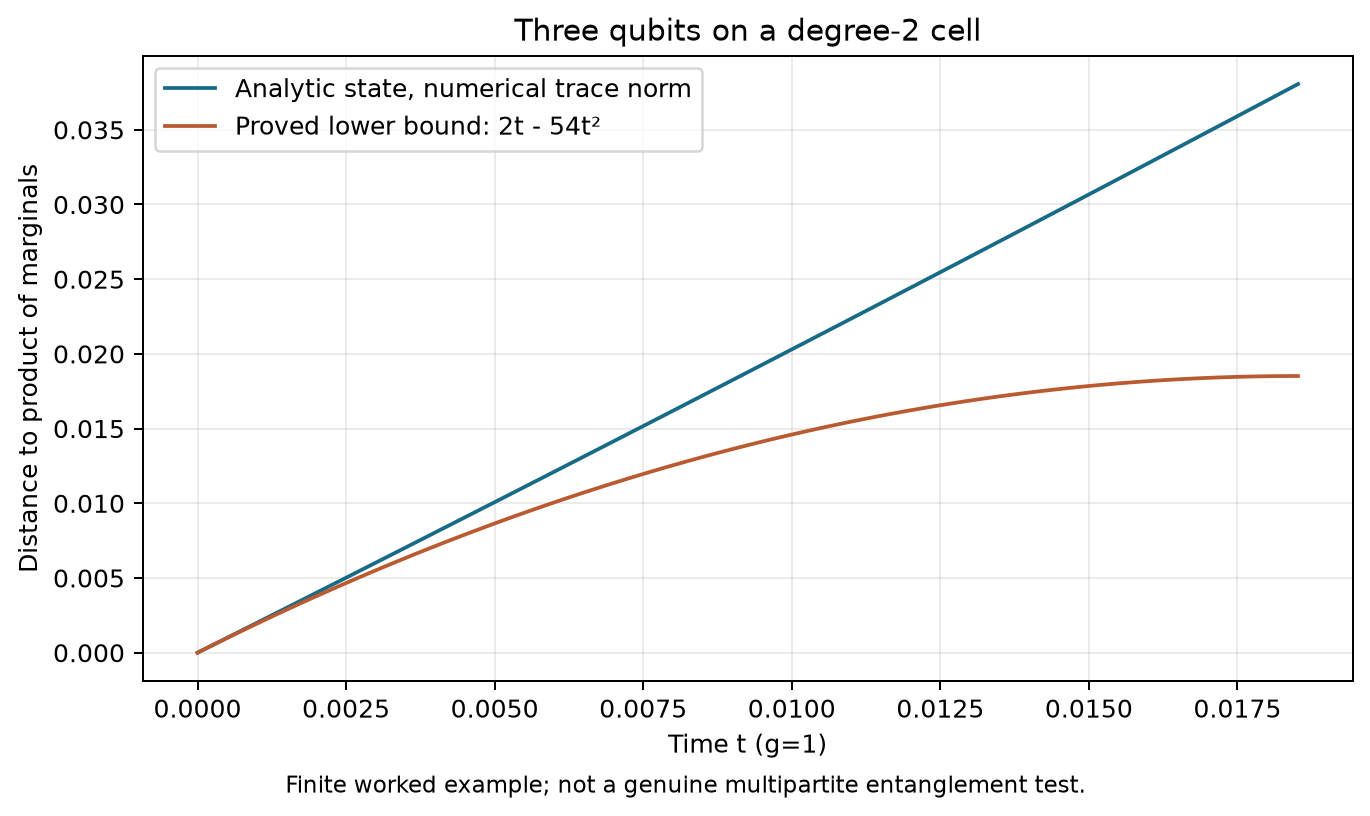
\includegraphics[keepaspectratio,alt={Three-qubit analytic-state defect and the proved lower bound for g=1.}]{public_export/fig1_overview.png}}
\caption{Three-qubit analytic-state defect and the proved lower bound for g=1.}
\end{figure}

\subsubsection{8.2 Evidence inventory}\label{evidence-inventory}

\begin{longtable}[]{@{}
  >{\raggedright\arraybackslash}p{(\linewidth - 4\tabcolsep) * \real{0.3333}}
  >{\raggedright\arraybackslash}p{(\linewidth - 4\tabcolsep) * \real{0.3333}}
  >{\raggedright\arraybackslash}p{(\linewidth - 4\tabcolsep) * \real{0.3333}}@{}}
\toprule\noalign{}
\begin{minipage}[b]{\linewidth}\raggedright
Result
\end{minipage} & \begin{minipage}[b]{\linewidth}\raggedright
Evidence in this package
\end{minipage} & \begin{minipage}[b]{\linewidth}\raggedright
Limit
\end{minipage} \\
\midrule\noalign{}
\endhead
\bottomrule\noalign{}
\endlastfoot
Projector algebra & Theorem 4.1; abstract Lean declarations; numerical tests & Lean assumes trace/embedding identities as structure fields \\
One-site isolation & Theorem 4.2; abstract one-site Lean declarations & No formal proof of all proper-support isolation \\
Highest-order isolation & Proposition 4.2b; numerical regressions & Separate projector, not a formal density-matrix instantiation \\
Short-time bound & Theorem 4.3; analytic-state comparisons & Entire-Hamiltonian norm hypothesis; code uses the weaker coefficient; not mechanized \\
Site-budget refinement & Lemma 4.3a; exact symbolic witness & Global norm remains in the coefficient; closed system; not mechanized \\
Reduced-subsystem bound & Lemma 4.3b; exact symbolic witness & Dilation norm remains; not a general Lindblad theorem; not mechanized \\
Jump trajectory without a finite dilation & Lemma 4.3c; exact scalar witness & One generator only; scalar coefficient 6; not mechanized \\
Finite jump family & Lemma 4.3d; comparison with Lemma 4.3c & Coefficient \(2(1+k^2)G^2\); no Hamiltonian; no site budgets; 10 rather than 6 on Lemma 4.3c; not mechanized \\
Hamiltonian beside jumps & Lemma 4.3e; commuting witness & Coefficient \(2(1+k^2)(g+G)^2\); 40 rather than 6 on the witness; cross term kept; no site budgets; not mechanized \\
Acceleration cross term & Lemma 4.3f; exact product witness & \(\|\rho''(0)\|_1=10>8=4(g^2+G^2)\); defect coefficient unchanged; \(\nu=0\); not mechanized \\
Polar witness & Theorem 4.4; numerical SVD & No automatic tangent-annihilator property \\
Hodge decomposition & Theorem 5.2; scalar incidence matrices & No sheaf or quantum-entanglement bridge \\
Square / semigroup defects & Separate derivations and regression examples & No automatic identification between the two \\
Protocol scaffold & Metadata and policy checks & No executed DDC simulation or authority \\
\end{longtable}

The Lean package is pinned to Lean 4.34.1. Its seven named declarations
establish consequences of the supplied abstract trace/embedding laws.
The axiom report's ``no axioms'' output means no global logical axioms appear
in those declarations; it does \textbf{not} remove their explicit structure
hypotheses. It is a stored report, not a fresh build receipt for this review.
The concrete density-matrix instantiation remains unmechanized.

The Python core uses NumPy floating-point linear algebra. It is not an
exact rational certifier, and there is no Rust implementation in this deposit.

The review receipt records executed tests, notebook execution method,
rendering checks, source identities, and any unavailable release gates.
A direct Python notebook-cell replay is distinct from a native Jupyter
kernel replay. Checksums establish byte identity, not theorem correctness
or publication status.

\subsubsection{8.3 Study route and remaining obligations}\label{study-route-and-remaining-obligations}

Lemma 4.3a is the closed-system site-budget refinement. Lemma 4.3b is
its finite-dilation extension to a reduced subsystem, including the
decoupled case in which the environment Hamiltonian drops out of the
reduced trajectory. Neither lemma removes the global factor \(g\).
Lemma 4.3c is one jump trajectory with no finite autonomous Hermitian dilation.
Its coefficient \(6\) is scalar. Lemma 4.3d gives the coefficient
\(2(1+k^2)G^2\) for a finite family of jumps and no Hamiltonian, where
\(G\) bounds the sum of the squared operator norms of the jumps. On the
Lemma 4.3c data this coefficient equals \(10\) and the half-speed window
is \(1/5\), against \(6\) and \(1/3\). The first-derivative budget \(2G\)
is achieved on that example; the quadratic coefficient is not sharp there.
Neither lemma replaces \(g\) by \(\max_j g_j\). Jump supports do not enter
Lemma 4.3d. Lemma 4.3d does not assert that a general jump trajectory
lacks a finite autonomous Hermitian dilation.
Lemma 4.3e places a Hamiltonian of operator norm at most \(g\) beside
that jump family. The quadratic coefficient is \(2(1+k^2)(g+G)^2\), from
the triangle bound \(\|\mathcal L(X)\|_1\le 2(g+G)\|X\|_1\). The cross
term inside \((g+G)^2\) is not removed. On the commuting witness with
\(g=G=1\) and \(k=2\), the coefficient is \(40\) and the half-speed
window is \(1/20\), against the scalar coefficient \(6\) and the window
\(1/3\). The first-derivative budget \(2(g+G)\) is not achieved there.
Site budgets still do not enter, and the scalar coefficient \(6\) is not
claimed for the family.
Lemma 4.3f is the acceleration witness for that cross term. With
\(g=G=1\), \(\|\rho''(0)\|_1=10\), strictly larger than
\(4(g^2+G^2)=8\) and strictly smaller than \(4(g+G)^2=16\). The orbit
is a product, so \(\nu=0\) and \(D(t)=0\). Substituting \(g^2+G^2\) into
the acceleration estimate is false. Whether the defect coefficient
\(2(1+k^2)(g+G)^2\) can be replaced by \(2(1+k^2)(g^2+G^2)\) through
some other argument is not settled.
Remaining obligations are a concrete Lean matrix model, fresh pinned Lean
replay, native notebook-kernel replay, removal of the global factor from
the quadratic coefficient, a mixed defect coefficient strictly smaller
than \(2(1+k^2)(g+G)^2\) by an argument other than the acceleration
substitution ruled out in Lemma 4.3f, a site-budget form of the jump
bound, a supplied sheaf coefficient system, and any proved observation
map linking quantum residual dynamics to cochain invariants.
These are stated as unfinished work.

\subsection{9. References and related repository material}\label{references-and-related-repository-material}

\begin{enumerate}
\def\labelenumi{\arabic{enumi}.}
\tightlist
\item
  Lim, L.-H. \emph{Hodge Laplacians on graphs}. arXiv:1507.05379 (2015; revised 2019).
  \href{https://arxiv.org/abs/1507.05379}{Primary manuscript}.
  Background for the finite Hodge viewpoint; it does not establish a
  quantum-entanglement interpretation here.
\item
  Haegeman, J., Lubich, C., Oseledets, I., Vandereycken, B., and Verstraete, F.
  \emph{Unifying time evolution and optimization with matrix product states}.
  Physical Review B 94, 165116 (2016).
  \href{https://doi.org/10.1103/PhysRevB.94.165116}{DOI};
  \href{https://arxiv.org/abs/1408.5056}{author preprint}.
  Context for variational tangent-space evolution, not a proof of this
  product-density bound.
\item
  Hall, M. J. W. \emph{Correlation Distance and Bounds for Mutual Information} (2013).
  \href{https://arxiv.org/html/1307.2697v1}{Primary manuscript}.
  Defines the same two-party correlation distance and gives the two-qubit
  sufficient entanglement criterion at distance greater than one.
\item
  Aaronson, B., Lo Franco, R., Compagno, G., and Adesso, G.
  \emph{Hierarchy and dynamics of trace distance correlations}.
  New Journal of Physics 15, 093022 (2013).
  \href{https://arxiv.org/abs/1307.3953}{Primary manuscript}.
  Distinguishes the closest product state from the product of marginals.
\item
  Carroll, J. H. \emph{Projection Obstruction repository series}.
  Repository collection.
  Related working papers motivate residual/cochain separation and
  projection-memory diagnostics. Their versions and deposition identities
  are not inferred from this package.
\end{enumerate}

\end{document}
